% This LaTeX document needs to be compiled with XeLaTeX.
\documentclass[
  10
]{article}
\usepackage[margin=2cm,includehead=true,includefoot=true,centering,]{geometry}
\usepackage{xcolor}
\usepackage{ucharclasses}
\usepackage{hyperref}
\usepackage{amsmath,amssymb}
\usepackage{amsfonts}
\usepackage[version=4]{mhchem}
\usepackage{stmaryrd}
\usepackage{bbold}
\usepackage{polyglossia}
\usepackage{fontspec}
\usepackage{ctex}
\usepackage[export]{adjustbox}
\usepackage{tabularx}
\usepackage{booktabs}

\usepackage{setspace}
\setstretch{1.2}

\makeatletter
\@ifundefined{KOMAClassName}{% if non-KOMA class
  \IfFileExists{parskip.sty}{%
    \usepackage{parskip}
  }{% else
    \setlength{\parindent}{0pt}
    \setlength{\parskip}{6pt plus 2pt minus 1pt}}
}{% if KOMA class
  \KOMAoptions{parskip=half}}
\makeatother
\usepackage{longtable,booktabs,array}
\newcounter{none} % for unnumbered tables
\usepackage{calc} % for calculating minipage widths
% Correct order of tables after \paragraph or \subparagraph
\usepackage{etoolbox}
\makeatletter
\patchcmd\longtable{\par}{\if@noskipsec\mbox{}\fi\par}{}{}
\makeatother
% Allow footnotes in longtable head/foot
\IfFileExists{footnotehyper.sty}{\usepackage{footnotehyper}}{\usepackage{footnote}}
\makesavenoteenv{longtable}
\usepackage{graphicx}
\makeatletter
\newsavebox\pandoc@box
\newcommand*\pandocbounded[1]{% scales image to fit in text height/width
  \sbox\pandoc@box{#1}%
  \Gscale@div\@tempa{\textheight}{\dimexpr\ht\pandoc@box+\dp\pandoc@box\relax}%
  \Gscale@div\@tempb{\linewidth}{\wd\pandoc@box}%
  \ifdim\@tempb\p@<\@tempa\p@\let\@tempa\@tempb\fi% select the smaller of both
  \ifdim\@tempa\p@<\p@\scalebox{\@tempa}{\usebox\pandoc@box}%
  \else\usebox{\pandoc@box}%
  \fi%
}
% Set default figure placement to htbp
\def\fps@figure{htbp}
\makeatother
\setlength{\emergencystretch}{3em} % prevent overfull lines
\providecommand{\tightlist}{%
  \setlength{\itemsep}{0pt}\setlength{\parskip}{0pt}}


\hypersetup{colorlinks=true, linkcolor=blue, filecolor=magenta, urlcolor=cyan,}
\urlstyle{same}

\usepackage{colortbl}
\definecolor{table-row-color}{HTML}{999999}
\definecolor{table-rule-color}{HTML}{999999}
%\arrayrulecolor{black!40}
\arrayrulecolor{table-rule-color}     % color of \toprule, \midrule, \bottomrule
\setlength{\aboverulesep}{0pt}
\setlength{\belowrulesep}{0pt}


\setotherlanguages{english}
\IfFontExistsTF{Source Han Serif CN}
{\newfontfamily\chinesefont{Source Han Serif CN}}
{\IfFontExistsTF{Noto Serif CJK SC}
  {\newfontfamily\chinesefont{Noto Serif CJK SC}}
  {\IfFontExistsTF{SimSun}
    {\newfontfamily\chinesefont{SimSun}}
    {\IfFontExistsTF{FangSong}
      {\newfontfamily\chinesefont{FangSong}}
      {\newfontfamily\chinesefont{Arial Unicode MS}}
}}}
\IfFontExistsTF{Times New Roman}
{\newfontfamily\englishfont{Times New Roman}}
{\IfFontExistsTF{Liberation Serif}
  {\newfontfamily\englishfont{Liberation Serif}}
  {\IfFontExistsTF{DejaVu Serif}
    {\newfontfamily\englishfont{DejaVu Serif}}
    {\newfontfamily\englishfont{Arial}}
}}


\author{}
\date{}

\begin{document}


\section{黄冈名卷}\label{ux9ec4ux5188ux540dux5377}

\section{第一单元知识回顾与检测}\label{ux7b2cux4e00ux5355ux5143ux77e5ux8bc6ux56deux987eux4e0eux68c0ux6d4b}

\subsection{圆}\label{ux5706}

\pandocbounded{
\includegraphics[keepaspectratio]{images/a7ae5459ccf245f66f8059955bf2286f73c9c8cdc8244823e4342064843a60c3.jpg}}

满分:100 分 时间:60 分钟

{\def\LTcaptype{none} % do not increment counter
\begin{longtable}[]{@{}|l|l|l|l|l|l|l|l|l|@{}}
\toprule\noalign{}
\endhead
\bottomrule\noalign{}
\endlastfoot
\hline
题 号 & 一 & 二 & 三 & 四 & 五 & 六 & 附加题 & 总 分 \\
\hline
得 分 & & & & & & & & \\
\hline
\end{longtable}
}

\subsection{一、填空。（22分）}\label{ux4e00ux586bux7a7a22ux5206}

\begin{enumerate}
\def\labelenumi{\arabic{enumi}.}
\tightlist
\item
  从( )到( )任意一点的线段叫作半径;通过( )并且两端都在(
  )的线段叫作直径。在同一个圆里,直径的长度是半径的( )。\\
\item
  画圆时, 圆规针尖固定的一点是圆的( ), 它决定圆的( ),
  圆规的两脚叉开的距离是所画圆的( ), 它决定圆的( )。\\
\item
  一个车轮转动一周,前进多少米是指圆的( )。\\
\item
  把一张圆形纸片至少折( )次, 就可以找到圆心。\\
\item
  用圆规画一个直径为 16 厘米的圆, 圆规两脚之间的距离是( )厘米,
  所画圆的周长是( )厘米, 面积是( )平方厘米。\\
\item
  在一个周长是 8 分米的正方形纸片上剪一个最大的圆, 这个圆的直径是 ( )
  分米, 面积是 ( ) 平方分米。\\
\item
  大圆半径是小圆半径的 2 倍, 大圆面积比小圆面积多 12 平方厘米,
  小圆面积是( )平方厘米。\\
\item
  一个圆的半径扩大为原来的 2 倍, 它的周长扩大为原来的 ( ) 倍,
  面积扩大为原来的 ( ) 倍。\\
\item
  把一个圆分成若干等份, 剪开拼成一个近似的长方形。这个长方形的长相当于(
  ), 长方形的宽就是圆的( )。\\
\item
  最早解决``轮子滚动的距离与轮子直径之间关系''的方案是(
  )，而这种方法往往因精确程度不够,影响计算圆周率的精确程度。
\end{enumerate}

\subsection{二、判断。(10 分)}\label{ux4e8cux5224ux65ad10-ux5206}

\begin{enumerate}
\def\labelenumi{\arabic{enumi}.}
\item
  圆周率与圆的大小有关。\\
\item
  两个圆的半径相等, 它们的周长相等, 面积也一定相等。 ( )
\item
  将一个圆形铁丝圈拉成长方形, 长方形与原来圆的周长相等。（）\\
\item
  直径为 5 厘米的圆比半径为 3 厘米的圆面积大。 （）\\
  5.两端都在圆上的所有线段中,直径是最长的一条。()
\end{enumerate}

\subsection{三、选择。(10 分)}\label{ux4e09ux9009ux62e910-ux5206}

\begin{enumerate}
\def\labelenumi{\arabic{enumi}.}
\tightlist
\item
  下面三种图形中, 对称轴最多的图形是( )。
\end{enumerate}

A. 长方形

B. 正方形

C. 圆

\begin{enumerate}
\def\labelenumi{\arabic{enumi}.}
\setcounter{enumi}{1}
\tightlist
\item
  两个直径不同的圆, 它们的周长( )。
\end{enumerate}

A.相等

B. 不相等

C. 有时相等

\begin{enumerate}
\def\labelenumi{\arabic{enumi}.}
\setcounter{enumi}{2}
\tightlist
\item
  在一张长 \(6 \, cm\) 、宽 \(4 \, cm\)
  的长方形纸中剪出一个最大的圆，这个圆的半径是（）。
\end{enumerate}

A. \(4 \mathrm{~cm}\)

B. \(6 \mathrm{~cm}\)

C. \(2 \mathrm{~cm}\)

\begin{enumerate}
\def\labelenumi{\arabic{enumi}.}
\setcounter{enumi}{3}
\tightlist
\item
  右图中, 三个圆的圆心在一条直线上, 那么大圆的周长(
  )两个小圆的周长之和。
\end{enumerate}

A. 大于

B. 等于

C. 小于

\begin{enumerate}
\def\labelenumi{\arabic{enumi}.}
\setcounter{enumi}{4}
\tightlist
\item
  在一个正方形里画一个最大的圆, 这个圆的面积是正方形面积的( )。
\end{enumerate}

A. \(\frac{1}{4}\)

B. \(\frac{3}{4}\)

C. \(\frac{\pi}{4}\)

\subsection{四、操作题。(22
分)}\label{ux56dbux64cdux4f5cux989822-ux5206}

\begin{enumerate}
\def\labelenumi{\arabic{enumi}.}
\tightlist
\item
  以 O 点为圆心, 画一个直径是 3 cm 的圆。(4 分)
\end{enumerate}

• O

\begin{enumerate}
\def\labelenumi{\arabic{enumi}.}
\setcounter{enumi}{1}
\tightlist
\item
  分别画出下面图形的对称轴。(4分)
\end{enumerate}

\pandocbounded{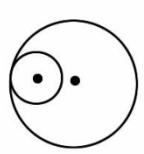
\includegraphics[keepaspectratio]{images/0f4005637fa233533e9e4d62d562d46851e2af19d85fa06505819e1f2595c463.jpg}}

\pandocbounded{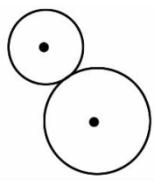
\includegraphics[keepaspectratio]{images/a8053eccda8047d8422f995656214f9312db5099b7f42d9dfbbeadfcd1053887.jpg}}

\pandocbounded{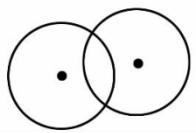
\includegraphics[keepaspectratio]{images/5a8421402849f49f2d8a6378ea90a69f352757c421f5f3dc6a93f63908bba716.jpg}}

\pandocbounded{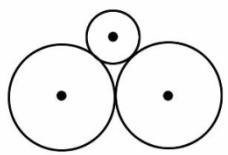
\includegraphics[keepaspectratio]{images/6bdbdf46d9324637e2dcedda4d28e201dbe7557659cc690a80e6f95a42cd7e42.jpg}}

\end{document}
